\documentclass{article}
\usepackage[hyphens]{url}
\usepackage{mathtools}
\usepackage{amsmath}
\usepackage{listings}
\usepackage{graphicx}
\usepackage[margin=1in]{geometry}
\usepackage{float}
\floatstyle{boxed}
\restylefloat{figure}
\lstset{breaklines=true}
\begin{document}


\title{CS595 Intro to Web Science, Assignment \#4}
\author{Valentina Neblitt-Jones}
\date{October 10, 2013}
\maketitle

\section*{Question 1}

From your list of 1000 links, choose 100 and extract all of the links from those 100 pages to other pages. We're looking for user navigable links, that is in the form of:  \\

\begin{verbatim}
<a href = "foo">bar</a>
\end{verbatim}

We're not looking for embedded images, scripts, <link> elements, etc. You'll probably want to use BeautifulSoup for this. \\

For each URI, create a text file of all the outbound links from that page to other URIs (use any syntax that is easy for you). For example: \\

site:
\url{http://www.cs.odu.edu/~mln/}

links:
\url{http://www.cs.odu.edu/}
\url{http://www.odu.edu}
\url{http://www.cs.odu.edu/~mln/research/}
\url{http://www.cs.odu.edu/~mln/pubs/}
\url{http://ws-dl.blogspot.com/}
\url{http://ws-dl.blogspot.com/2-13/09/2013-09-09-ms-thesis-http-mailbox.html}
etc. \\

Upload these 100 files to github (they don't have to be in your report).

\subsection*{Answer to Question 1}

%\begin{figure}[H]
%\centering
%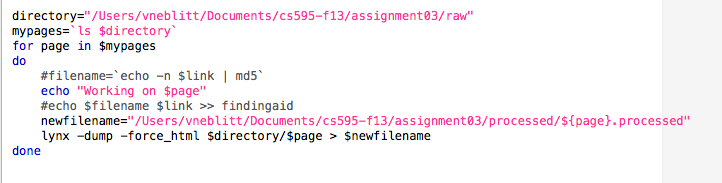
\includegraphics[scale=0.50]{q1/rmMarkupURI}
%\caption{Shell Script to Remove Markup}
%\label{rmMarkup}
%\end{figure}

\newpage

\section*{Question 2}

Using these 100 files, create a single GraphViz ``dot'' file of the resulting graph. Learn about dot at: \\

Examples:
\begin{itemize}
\item \url{http://www.graphviz.org/content/unix}
\item \url{http://www.graphviz.org/Gallery/directed/unix.gv.txt}
\end{itemize}

Manual:
\begin{itemize}
\item \url{http://www.graphviz.org/Documentation/dotguide.pdf}
\end{itemize}

Reference:
\begin{itemize}
\item \url{http://www.graphviz.org/content/dot-language}
\item \url{http://www.graphviz.org/Documentation.php}
\end{itemize}

Note: You'll have to put explicit labels on the graph, see: \url{https://gephi.org/users/supported-graph-formats/graphviz-dot-format/} \\

Note: Actually, I'll allow any of the formats listed here: \url{https://gephi.org/users/supported-graph-formats/}, but ``dot'' is probably the simplest.

%\begin{table}[!h]
%\centering
%\caption{10 Hits for the term ``shadow'', ranked by TFIDF}
%\begin{tabular}{c c c c}
%\hline
%TFIDF & TF & IDF & URI \\
%\hline
%\hline
%0.150 & 0.014 & 10.680 & http://foo.com \\
%0.085 & 0.008 & 10.680 & http://bar.com \\
%\hline
%\end{tabular}
%\end{table}

\subsection*{Answer to Question 2}


\clearpage

\section*{Question 3}
Download and install Gephi: \\
\url{}

Load the dot file created in \#2 and use Gephi to:
\begin{itemize}
\item visualize the graph (you'll have to turn on labels)
\item calculate HITS and PageRank
\item avg degree
\item network diameter
\item connected components
\end{itemize}

Put the resulting graphs in your report. \\

You might need to choose the 100 sites with an eye toward creating a graph with at least one component that is nicely connected. You can probably do this be selecting some portion of your links (e.g., 25, 50) from the same site.

\subsection*{Answer to Question 3}

\end{document}